%%%%%%%%%%%%%%%%%%%%%%%%%%%%%%%%%%%%%%%%%
% Sullivan Business Report
% Adapted for recap-agent technical architecture report
%%%%%%%%%%%%%%%%%%%%%%%%%%%%%%%%%%%%%%%%%

\documentclass[
	a4paper,
	12pt,
]{CSSullivanBusinessReport}

\usepackage[spanish,es-tabla]{babel}
\usepackage{csquotes}
\usepackage{tabularx}
\usepackage{longtable}
\usepackage{tikz}
\usetikzlibrary{arrows.meta, positioning, shapes.geometric, shapes.misc, fit, calc}

\addbibresource{sample.bib}

\reporttitle{recap-agent}
\reportsubtitle{Informe técnico de arquitectura e implementación\\para un agente conversacional serverless}
\reportauthors{Sin Envolturas}
\reportdate{22 de junio de 2026}
\rightheadercontent{\small Informe técnico}

\hypersetup{
	pdftitle={recap-agent: informe técnico de arquitectura e implementación},
	pdfauthor={Sin Envolturas},
	colorlinks=true,
	linkcolor=DarkBlue,
	urlcolor=DarkBlue,
	citecolor=DarkBlue
}

\newcommand{\term}[1]{\textbf{#1}}
\newcommand{\smallcaps}[1]{\textsc{#1}}
\newcommand{\metric}[1]{\textsf{#1}}
\newcommand{\component}[1]{\textsf{#1}}
\newcommand{\brandlogo}[2]{%
	\IfFileExists{Images/#1}{%
		\includegraphics[height=0.75cm,keepaspectratio]{Images/#1}%
	}{%
		\fbox{\parbox[c][0.62cm][c]{2.8cm}{\centering\scriptsize #2\\placeholder}}%
	}%
}

\makeatletter
\newcommand{\ps@recaplogos}{%
	\renewcommand{\@oddhead}{\brandlogo{utec-logo.png}{UTEC}\hfill\small Informe técnico\hfill\brandlogo{sin-envolturas-logo.jpeg}{Sin Envolturas}}%
	\renewcommand{\@evenhead}{\@oddhead}%
	\renewcommand{\@oddfoot}{\hfill\thepage\hfill}%
	\renewcommand{\@evenfoot}{\@oddfoot}%
}
\makeatother

\tikzset{
	box/.style={draw=DarkBlue, rounded corners=2pt, very thick, align=center, inner sep=6pt, fill=AliceBlue},
	store/.style={draw=DarkGreen, rounded corners=2pt, very thick, align=center, inner sep=6pt, fill=Honeydew},
	ext/.style={draw=DarkRed, rounded corners=2pt, very thick, align=center, inner sep=6pt, fill=MistyRose},
	agent/.style={draw=DarkOrange, rounded corners=2pt, very thick, align=center, inner sep=6pt, fill=OldLace},
	decision/.style={draw=DarkMagenta, diamond, aspect=2.1, very thick, align=center, inner sep=2pt, fill=LavenderBlush},
	flow/.style={-{Latex[length=3mm]}, very thick, draw=DimGray},
	dashedflow/.style={-{Latex[length=3mm]}, very thick, dashed, draw=DimGray}
}

\begin{document}
\pagestyle{recaplogos}

\thispagestyle{empty}
\begin{fullwidth}
	\vspace*{-0.06\textheight}
	\brandlogo{utec-logo.png}{UTEC}\hfill\brandlogo{sin-envolturas-logo.jpeg}{Sin Envolturas}

	\vspace{0.14\textheight}

	\parbox{0.9\fulltextwidth}{\fontsize{48pt}{50pt}\selectfont\raggedright\textbf{\reporttitle}\par}

	\vspace{0.03\textheight}

	{\LARGE\textit{\textbf{\reportsubtitle}}\par}

	\vfill

	{\Large Sin Envolturas\par}

	\vfill\vfill\vfill

	{\large\reportdate\par}
\end{fullwidth}

\newpage

\thispagestyle{empty}
\begin{twothirdswidth}
	\footnotesize

	\subsection*{Resumen documental}

	Este informe consolida la arquitectura y la implementación de \textit{recap-agent}, un prototipo funcional de agente conversacional para la recomendación de proveedores de eventos en Sin Envolturas. La redacción toma como criterio formal la precisión, concisión, claridad y revisión objetiva recomendadas para informes técnicos \cite{unam-informe-tecnico}; el análisis técnico se fundamenta en la revisión integral del repositorio del proyecto, la bitácora de implementación, la documentación operativa y de evaluación, y los expedientes de análisis generados durante el desarrollo. Además, se consideran los artefactos de alcance y diseño, junto con la verificación del despliegue de desarrollo en AWS utilizando el perfil autorizado del proyecto.

	\subsection*{Alcance}

	El documento describe el sistema en términos de arquitectura, contratos, decisiones técnicas, modelo de dominio, persistencia, integración con proveedores, conocimiento, despliegue, telemetría y evaluación. No reproduce fragmentos de implementación ni depende de rutas de archivos como mecanismo explicativo; el énfasis está en el diseño técnico resultante y en las decisiones que lo sustentan.

	\subsection*{Control de cambios}

	\scriptsize
	\begin{tabular}{@{} L{0.08\linewidth} L{0.18\linewidth} L{0.58\linewidth} @{}}
		\toprule
		v1.0 & 2026-06-22 & Informe inicial elaborado a partir del código vigente, artefactos de diseño del proyecto, expedientes de análisis y despliegue AWS de desarrollo.\\
		\bottomrule
	\end{tabular}
\end{twothirdswidth}

\newpage

\begin{twothirdswidth}
	\tableofcontents
\end{twothirdswidth}

\newpage

\section{Introducción}

\textit{recap-agent} es un prototipo funcional de agente conversacional para Sin Envolturas. Este desarrollo surge ante la necesidad de optimizar la experiencia de usuarios que planifican eventos, facilitando la identificación y selección de proveedores adecuados mediante un enfoque conversacional innovador. El problema que aborda no es la negociación final del servicio, sino la etapa previa de conversación, estructuración de requisitos, búsqueda, shortlist y generación de contacto. En términos de producto, el agente reduce la distancia entre una solicitud informal --por ejemplo, ``necesito ayuda para una boda en Lima''-- y una acción útil sobre el marketplace: identificar necesidades, consultar proveedores reales, explicar opciones y cerrar una solicitud cuando el usuario decide avanzar. Este enfoque se relaciona con la literatura reciente sobre recomendadores conversacionales en preventa, donde los modelos de lenguaje y los sistemas de recomendación resultan complementarios para comprender preferencias y apoyar decisiones de compra \cite{liu-2023-crs-llm}. A diferencia de soluciones tradicionales, \textit{recap-agent} integra capacidades de lenguaje natural y búsqueda semántica, permitiendo una interacción más flexible y personalizada en la etapa de preventa.

Para abordar estos desafíos, el proyecto formula el objetivo como el diseño e implementación de un agente integrado con las APIs de Sin Envolturas, capaz de entrevistar usuarios por WhatsApp, estructurar requisitos y recomendar proveedores relevantes. Este alcance introduce una restricción importante: el canal inicial se comporta como WhatsApp, por lo que la respuesta debe ser síncrona, breve y no dependiente de streaming. Al mismo tiempo, la solución no puede quedar acoplada a WhatsApp, porque la evolución natural del sistema incluye webchat, terminal de evaluación y otros canales.

Durante el diseño temprano se descartó una hipótesis demasiado optimista: que OpenAI pudiera hospedar toda la integración con WhatsApp y con las APIs internas sin una capa propia. La decisión vigente separa canal, adaptación, runtime conversacional e integraciones de negocio. Así, OpenAI provee capacidades de interpretación, extracción y generación, mientras que el proyecto conserva un runtime propio para controlar estado, herramientas, persistencia, observabilidad y validaciones. Esta separación coincide con la orientación de la plataforma de agentes de OpenAI, que ubica a los agentes como aplicaciones capaces de planificar, usar herramientas y mantener estado bajo control de la aplicación que los integra \cite{openai-agents-sdk}.

El análisis y las conclusiones presentadas en este informe se fundamentan en la implementación vigente del repositorio como fuente autoritativa, complementada con la bitácora de implementación, documentación operativa, expedientes de análisis, artefactos de diseño del proyecto y verificación del despliegue AWS de desarrollo con el perfil \textit{se-dev}.

\section{Arquitectura del sistema}

La arquitectura implementada organiza el sistema en torno a un límite simple: el runtime recibe un turno normalizado y devuelve una respuesta normalizada. El adaptador de canal se encarga de la identidad externa, autenticación del webhook, idempotencia y entrega al usuario. El núcleo conversacional, por su parte, solo necesita conocer el texto entrante, el canal, el usuario externo y metadatos de sesión. Esa frontera permite que WhatsApp, un web client o la terminal de pruebas consuman el mismo contrato sin modificar el flujo interno.

La Figura \ref{fig:aws-architecture} presenta la vista física recomendada para documentar el despliegue. El diagrama distingue los usuarios y canales de entrada, el límite serverless de AWS, la capa de agente en OpenAI y las APIs de Sin Envolturas que alimentan la recomendación y la sincronización. La función principal vive en AWS Lambda y se expone en desarrollo mediante Function URL, un endpoint HTTPS dedicado para una función Lambda \cite{aws-lambda-function-urls}. DynamoDB mantiene planes y telemetría como base NoSQL administrada \cite{aws-dynamodb-introduction}; Secrets Manager conserva la credencial de OpenAI \cite{aws-secrets-manager}; CloudWatch centraliza logs operativos \cite{aws-cloudwatch-logs}; S3 almacena artefactos de sincronización \cite{aws-s3}; y EventBridge activa jobs periódicos para conocimiento y proveedores \cite{aws-eventbridge-scheduler}.

\begin{figure}[H]
\centering
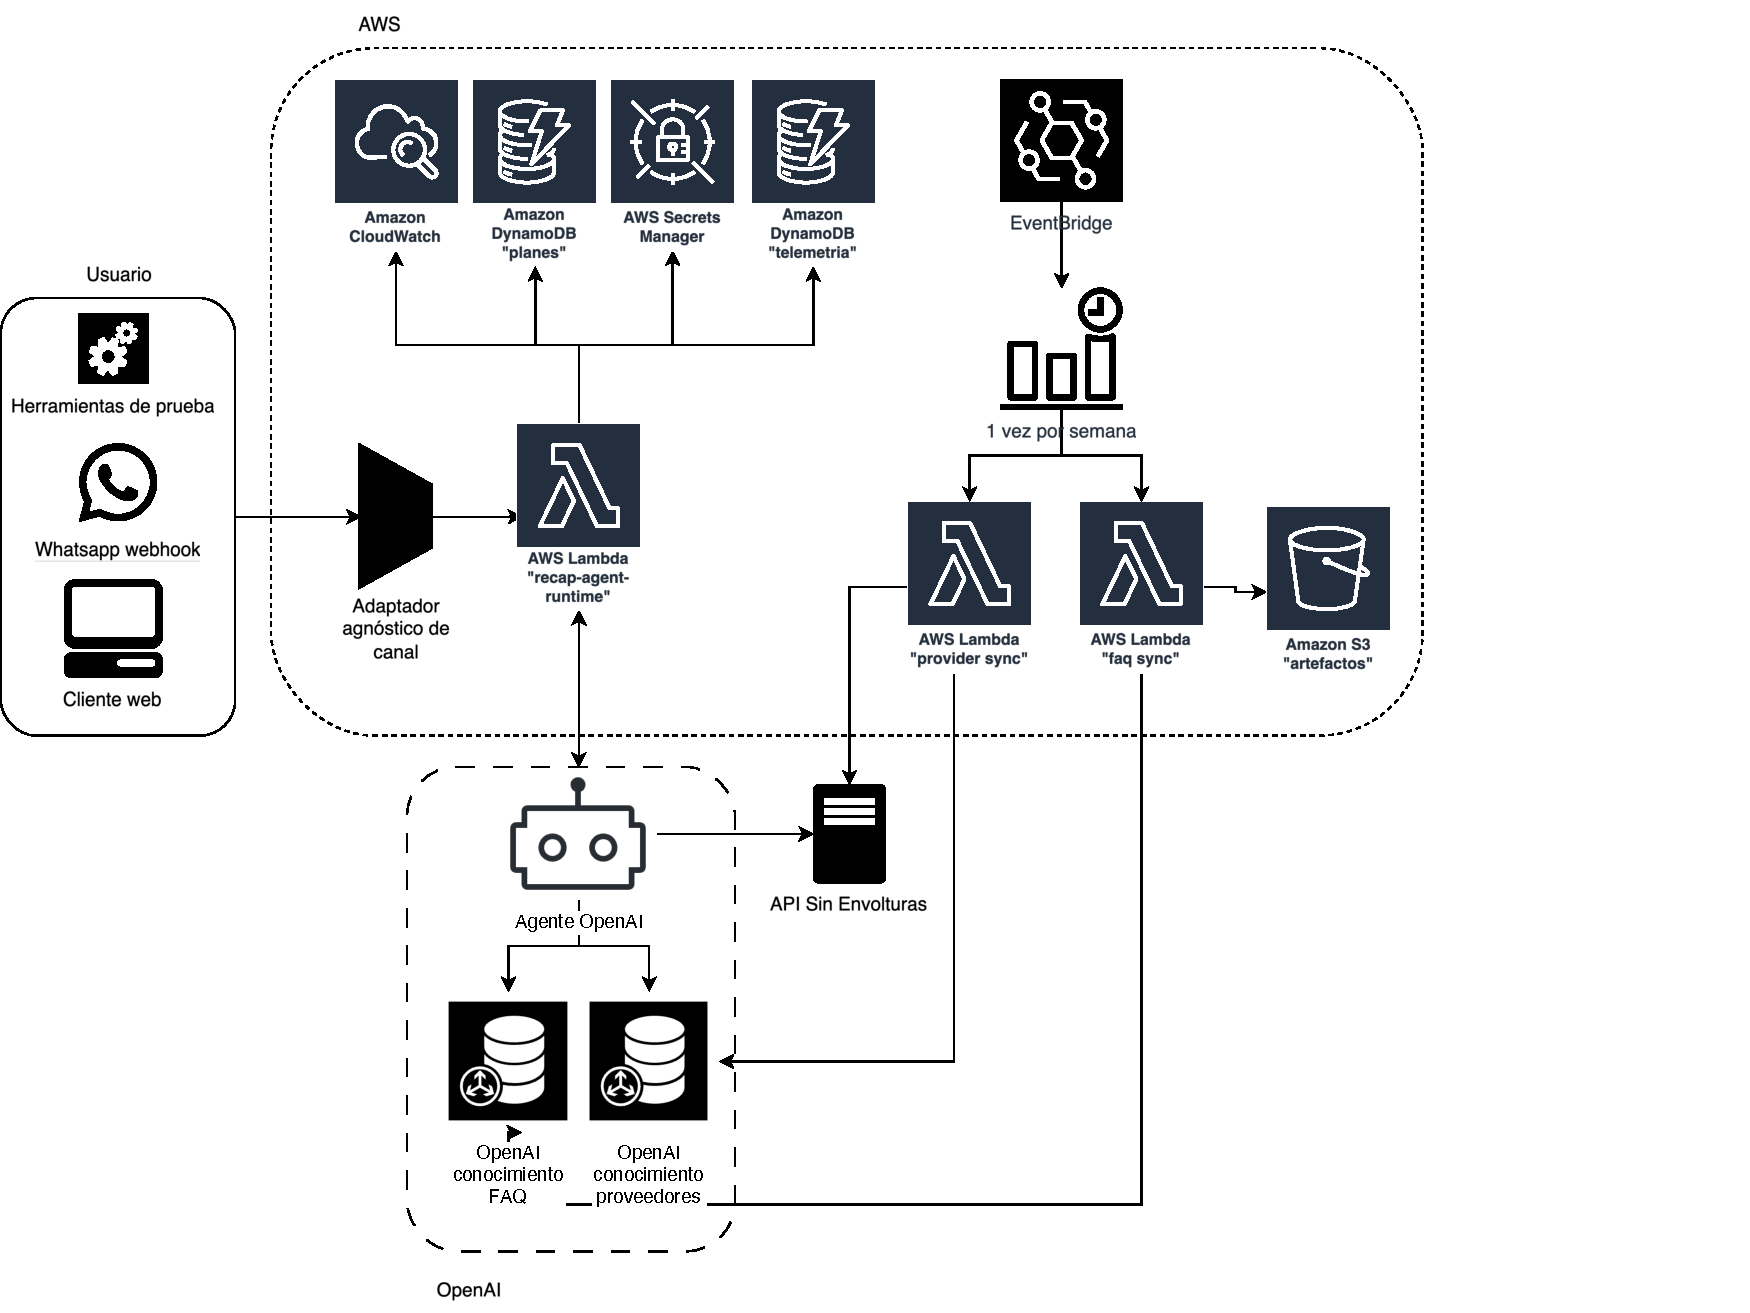
\includegraphics[width=\linewidth]{Images/architecture-diagram.pdf}
\caption{Vista de despliegue AWS y relación con canales, OpenAI y APIs de Sin Envolturas.}
\label{fig:aws-architecture}
\end{figure}

Como se ilustra en la Figura \ref{fig:aws-architecture}, la verificación realizada el 22 de junio de 2026 confirmó que el entorno de desarrollo cuenta con tres componentes principales desplegados y operativos:

\begin{itemize}
	\item \term{Runtime principal}: núcleo del agente conversacional, encargado de procesar las interacciones, coordinar la extracción estructurada, consultar herramientas y componer respuestas.
	\item \term{Sync de proveedores}: función dedicada a la actualización periódica de la información de proveedores desde las APIs de Sin Envolturas hacia el vector store de proveedores.
	\item \term{Sync de conocimiento}: mantiene actualizada la base usada para preguntas frecuentes e información operativa relevante.
\end{itemize}

El runtime principal fue actualizado el 19 de junio de 2026, opera en \textit{us-east-1}, usa modelos separados para respuesta y extracción, mantiene búsqueda híbrida, habilita FAQ y consulta de invitado, y conserva telemetría con TTL de 30 días. Los stacks auxiliares mantienen los vector stores de proveedores y conocimiento que el runtime consume.

En la implementación, esta arquitectura se traduce en una separación de responsabilidades. La entrada serverless valida la solicitud y delega la conversación. El runtime orquesta extracción, estado, herramientas y respuesta. El dominio define el plan, las necesidades, las transiciones y la evidencia. Las integraciones encapsulan APIs externas, búsqueda semántica, creación de cotizaciones y sincronización. La capa de almacenamiento conserva planes y métricas por turno. Esta división evita que la lógica de WhatsApp, la generación de lenguaje y la persistencia del plan queden entremezcladas.

\section{Modelo conversacional y estado}

El comportamiento del agente se diseñó como una entrevista guiada pero no rígida. La intención original del flujo era transformar lenguaje natural en requisitos estructurados y decidir cuándo consultar herramientas para recomendar de manera útil y trazable. La implementación materializa esa idea mediante una máquina de estados tipada, es decir, un modelo formal que define explícitamente los posibles estados de la conversación y las transiciones permitidas entre ellos. Esto permite controlar el flujo sin que el usuario perciba rigidez, ya que puede aportar información en cualquier orden. El agente puede aceptar información libre, reutilizar contexto previo, pedir solo los faltantes críticos y recomendar con supuestos explícitos cuando ya existe suficiencia mínima. Por ejemplo, si el usuario primero indica la ciudad y luego el tipo de evento, el agente puede conservar ambos datos, inferir restricciones iniciales de búsqueda y sugerir proveedores relevantes aunque todavía falten detalles como fecha exacta o número de invitados. Esta orientación responde a una tensión común en agentes conversacionales de producción: mantener flexibilidad lingüística sin perder restricciones de servicio, trazabilidad ni control operativo \cite{park-2025-workflow-graphs}.

La pieza central del estado es el plan de evento. Un plan conserva identidad, canal, usuario externo, ciclo de vida, nodo actual, intención, tipo de evento, ubicación, presupuesto, escala de invitados, preferencias, restricciones, preguntas abiertas, resumen conversacional y datos de contacto. Lo más importante es que el plan puede contener varias necesidades de proveedor. Una boda, por ejemplo, puede tener local, catering, música y fotografía como frentes distintos. Cada frente puede estar identificado, listo para búsqueda, con shortlist, seleccionado, aplazado o sin proveedores disponibles. Esta decisión \textit{event-plan-first} evita que una búsqueda nueva destruya selecciones anteriores.

La Figura \ref{fig:runtime-state} resume la relación entre interpretación, decisión y persistencia. El extractor produce evidencia estructurada; el runtime combina esa evidencia con el plan persistido; las reglas tipadas deciden el nodo operativo; las herramientas se habilitan por contexto; y el plan se guarda con la nueva evidencia. El diagrama no intenta enumerar todos los nodos, sino mostrar el ciclo estable que gobierna cada turno. En cada turno, el sistema sigue una secuencia estable: recibe la entrada del usuario, extrae evidencia estructurada, actualiza el plan persistente, decide el siguiente nodo según reglas tipadas, habilita herramientas contextuales, compone la respuesta y guarda el nuevo estado junto con la telemetría.

\begin{figure}[H]
\centering
\resizebox{\linewidth}{!}{%
\begin{tikzpicture}[x=1cm,y=1cm, every node/.style={font=\footnotesize}]
	\tikzset{
		rstep/.style={draw=DarkBlue, rounded corners=2pt, thick, fill=AliceBlue, align=center, minimum width=3.0cm, minimum height=0.85cm},
		model/.style={draw=DarkOrange, rounded corners=2pt, thick, fill=OldLace, align=center, minimum width=3.0cm, minimum height=0.85cm},
		state/.style={draw=DarkGreen, rounded corners=2pt, thick, fill=Honeydew, align=center, minimum width=3.0cm, minimum height=0.85cm},
		tool/.style={draw=DarkRed, rounded corners=2pt, thick, fill=MistyRose, align=center, minimum width=3.0cm, minimum height=0.85cm},
		arrow/.style={-{Latex[length=2.1mm]}, thick, draw=DimGray}
	}
	\node[rstep] (in) at (0,2.0) {Turno normalizado};
	\node[model] (extract) at (3.7,2.0) {Extractor\\estructurado};
	\node[state] (plan) at (7.4,2.0) {Plan persistente\\multi-necesidad};
	\node[rstep] (decision) at (11.1,2.0) {Decisión de nodo\\con evidencia};
	\node[tool] (tools) at (11.1,0.2) {Herramientas\\según contexto};
	\node[model] (reply) at (7.4,0.2) {Agente de respuesta\\en español};
	\node[rstep] (out) at (3.7,0.2) {Render y saneamiento\\del canal};
	\node[state] (save) at (0,0.2) {Guardado de plan\\y telemetría};

	\draw[arrow] (in) -- (extract);
	\draw[arrow] (extract) -- (plan);
	\draw[arrow] (plan) -- (decision);
	\draw[arrow] (decision) -- (tools);
	\draw[arrow] (tools) -- (reply);
	\draw[arrow] (decision) -- (reply);
	\draw[arrow] (reply) -- (out);
	\draw[arrow] (out) -- (save);
\end{tikzpicture}
}
\caption{Ciclo de interpretación, decisión y persistencia de un turno.}
\label{fig:runtime-state}
\end{figure}

Una restricción de ingeniería atraviesa todo este modelo: las decisiones conversacionales no se toman mediante palabras clave ni coincidencias exactas. El modelo interpreta y entrega evidencia estructurada, pero el runtime valida, normaliza y decide las consecuencias. Esta separación fue crucial para corregir fallos observados durante el desarrollo, como selección múltiple de proveedores, corrección parcial de datos de contacto, descarte de necesidades, recuperación de código de invitado y preservación de proveedores seleccionados. Además, garantiza que errores en la interpretación del lenguaje natural no comprometan la integridad del estado del plan, ya que toda decisión relevante se valida y normaliza antes de afectar el flujo conversacional. La conversación puede ser natural, pero el estado durable permanece tipado.

Los prompts también forman parte del contrato de arquitectura. Están versionados como texto, en español, y organizados por nodo de flujo. Cada nodo define objetivo, política de herramientas, contrato de respuesta y reglas de transición. El versionado de prompts permite auditar cambios en el comportamiento conversacional y facilita la experimentación controlada, asegurando que cada modificación pueda ser evaluada y revertida si es necesario.

\section{Integración con proveedores, conocimiento y cierre}

La recomendación de proveedores usa una estrategia híbrida. La API de Sin Envolturas sigue siendo la fuente de verdad para identificadores, enlaces, detalles, acciones de cotización y estado real. En paralelo, el vector store de proveedores agrega recuperación semántica sobre descripciones, servicios, promociones y términos. Este patrón se apoya en la idea de recuperación semántica sobre datos propios mediante vector stores, que permite encontrar resultados similares aunque no compartan exactamente las mismas palabras de la consulta \cite{openai-retrieval}. En modo híbrido, el runtime consulta información estructurada desde las APIs internas y utiliza el vector store para recuperar proveedores relevantes por similitud semántica. Los resultados se fusionan priorizando información completa y actualizada, se deduplican y se enriquecen antes de presentarse al agente de respuesta. La búsqueda vectorial no se expone como herramienta libre al modelo; se ejecuta dentro del runtime y produce una lista tipada de candidatos.

El aislamiento por necesidad es deliberado. Por ejemplo, si el usuario busca proveedores de música y luego de catering, las preferencias y filtros aplicados en la búsqueda de música no alteran los resultados ni las recomendaciones para catering, garantizando independencia y precisión en cada frente. Del mismo modo, la base de conocimiento de FAQ no se mezcla con la búsqueda de proveedores. La base de conocimiento se actualiza periódicamente a partir de fuentes operativas del proyecto y retroalimentación revisada; cada entrada se valida antes de incorporarse al vector store, asegurando respuestas precisas y verificables. Las preguntas sobre comisiones, soporte, listas de regalo o reclamos entran a un nodo de conocimiento que usa su propio vector store y preserva el plan de evento para que el usuario pueda volver a planificación después. Esta separación reduce falsos positivos y facilita explicar qué fuente intervino en cada respuesta; trabajos recientes sobre motores de diálogo con recuperación aumentada también resaltan la importancia de organizar el conocimiento de dominio para mejorar precisión y verificabilidad \cite{yu-2025-graphrag}.

La calidad del marketplace condiciona la precisión de las recomendaciones. Los expedientes de análisis muestran que, en la auditoría exhaustiva del 14 de abril de 2026, el sistema podía diferenciar proveedores en varias categorías, pero la cobertura de campos estructurados era desigual. Descripciones, promociones, servicios, términos, ubicación, precio y ratings no estaban completos de manera uniforme. Por ello, el agente justifica con la evidencia disponible y evita sobreafirmar cuando un proveedor tiene pocos datos comparativos.

El cierre del flujo también es una integración de negocio, no solo un mensaje final. Cuando el usuario selecciona proveedores y entrega contacto válido, el sistema crea solicitudes de cotización o contacto para esos proveedores. Antes de enviar una solicitud, el runtime valida en tiempo real el teléfono y el correo electrónico proporcionados. Si detecta un error, solicita al usuario corregir la información antes de proceder; así evita que datos inválidos lleguen tarde al endpoint de cotización y produzcan ciclos confusos. El cierre puede ser parcial: una necesidad aplazada o sin resultados no bloquea otra necesidad ya seleccionada. En cambio, una shortlist con opciones visibles y sin decisión exige selección o descarte explícito antes de cerrar.

\section{Persistencia, observabilidad y evaluación}

La persistencia se organiza por canal e identificador externo de usuario. Esto permite que la continuidad de conversación sea durable sin asumir que todos los canales comparten la misma identidad. El sistema utiliza identificadores de sesión y de usuario externo para distinguir conversaciones activas, reanudaciones y nuevas interacciones. El plan almacena el estado necesario para reanudar, pero el runtime también maneja foco de sesión para evitar que mensajes de sesiones previas influyan en nuevas conversaciones o que una interacción nueva herede contexto efímero de una conversación anterior. En paralelo, cada turno produce telemetría: ruta de nodos, herramientas consideradas, herramientas llamadas, resultados de proveedor, métricas de latencia, uso de tokens, resúmenes de extracción y estado de persistencia. Por ejemplo, la telemetría permite detectar incrementos de latencia durante consultas o sincronizaciones de proveedores y orientar optimizaciones en las rutas de búsqueda, persistencia o enriquecimiento.

La observabilidad evolucionó a partir de fallos reales. Al principio, las trazas permitían investigar estado y latencia, pero no siempre explicaban defectos de redacción final. La versión actual añade vista previa redactada de la respuesta, hash, flags de calidad y resúmenes de herramientas, todo con retención temporal. Esto permite investigar fugas de formato, mensajes robóticos o artefactos de cita sin depender únicamente de capturas manuales.

La evaluación evita comparar transcripciones completas, porque eso haría frágil la suite. En lugar de exigir una frase exacta, los casos verifican estado final, trayectoria, uso de herramientas, presencia o ausencia de proveedores, invariantes de selección, métricas de tokens y fragmentos contractuales. Hay un target offline con fixtures y almacenamiento en memoria, y un target live que llama al Lambda desplegado y confirma consumo real. Esta doble superficie permite iterar rápido y, al mismo tiempo, detectar drift entre la implementación local y el entorno real. La infraestructura se mantiene mediante CloudFormation, coherente con el uso de infraestructura como código para modelar y administrar recursos AWS como unidades de despliegue \cite{aws-cloudformation}.

Los contratos resumidos en la Tabla \ref{tab:contracts} se auditan mediante versionado de prompts, pruebas automatizadas, bitácora de implementación y trazas por turno. Esta combinación permite reconstruir qué cambió, por qué se cambió y qué comportamiento se verificó después, preservando trazabilidad entre arquitectura, conversación y despliegue.

\begin{table}[H]
\caption{Contratos principales del sistema.}
\label{tab:contracts}
\begin{tabularx}{\linewidth}{@{} L{0.24\linewidth} X @{}}
\toprule
\term{Contrato} & \term{Función arquitectónica}\\
\midrule
Turno normalizado & Desacopla WhatsApp, webchat, CLI y evaluación del runtime central.\\
Plan de evento & Mantiene estado durable, multi-necesidad, selección, contacto y resumen conversacional.\\
Extracción estructurada & Convierte lenguaje natural en evidencia validable para decisiones de flujo.\\
Herramientas por nodo & Limita qué integraciones pueden ejecutarse en cada contexto conversacional.\\
Telemetría por turno & Hace auditable la trayectoria, el costo, los resultados y la calidad de salida.\\
Suites de evaluación & Verifican comportamiento por estado y trayectoria, no por transcript rígido.\\
\bottomrule
\end{tabularx}
\end{table}

\section{Discusión}

La implementación muestra una evolución clara desde un agente de búsqueda hacia un runtime conversacional de dominio. La transición de una selección singular a una selección múltiple por necesidad permitió que los usuarios gestionaran eventos complejos sin perder información previa, mejorando la flexibilidad del flujo y reduciendo fricción cuando aparecen varios frentes de contratación. La separación entre la base de conocimiento y la búsqueda de proveedores disminuyó respuestas ambiguas, porque las preguntas operativas dejaron de competir con los resultados comerciales. La validación temprana de contacto, por su parte, trasladó los errores corregibles al momento conversacional adecuado, antes de crear solicitudes incompletas.

El principal riesgo técnico sigue siendo la calidad variable del marketplace. Para mitigarlo, el runtime prioriza una lógica de justificación basada en evidencia y evita sobreafirmar cuando faltan ubicación, precio, servicios o términos. El equipo puede reducir este riesgo ampliando la cobertura estructurada de proveedores y fortaleciendo las auditorías de datos antes de cada sincronización. Otro riesgo es la frontera de canal: la Function URL de desarrollo no autentica por sí misma, por lo que el adaptador productivo incorpora como trabajo necesario la validación de webhook, idempotencia, rate limits y políticas de abuso. Finalmente, las evaluaciones live consumen tokens y dependen de servicios externos; por ello, el proyecto las usa como complemento de la validación offline, no como sustituto de pruebas determinísticas.

En conjunto, \textit{recap-agent} es un prototipo defendible como artefacto de tesis porque combina una arquitectura serverless real, estado conversacional tipado, herramientas de negocio, búsqueda híbrida, conocimiento semántico y evaluación reproducible. Su valor no reside únicamente en generar texto, sino en sostener una conversación que puede convertirse en acciones verificables sobre un marketplace.

\section{Conclusiones}

El sistema responde a las restricciones iniciales del proyecto: opera de forma compatible con WhatsApp, conserva independencia de canal, consulta datos vivos, mantiene planes con múltiples necesidades y registra suficiente evidencia para evaluar decisiones. La arquitectura reconoce que OpenAI es una capa de inteligencia y orquestación, no el sistema completo de integración; por ello, el runtime propio conserva la autoridad sobre persistencia, validación, herramientas y cierre.

El estado actual permite presentar el proyecto como un prototipo funcional con base técnica sólida. Los siguientes pasos naturales son endurecer el adaptador productivo de WhatsApp, mejorar datos estructurados del marketplace, ampliar conversaciones de evaluación completas, incorporar métricas longitudinales de usuarios de prueba y producir una versión gráfica final de la arquitectura con iconografía oficial de AWS y OpenAI a partir de la topología descrita en este informe.

\printbibliography

\end{document}
